\documentclass[12pt]{article}
\usepackage{tikz}
\usepackage{ifthen}
\usetikzlibrary{arrows}

% type, redundancy, required, lambda 
\newcommand{\modelgraphlabel}[4]{$#1$ \\ $r=#2$ \\ $\nu=#3$ \\ $\lambda=#4$}

\begin{document}
% Cloud Model 
\begin{figure}
	% draw - outline, fill - color!alpha, align - allows for manual linebreak
	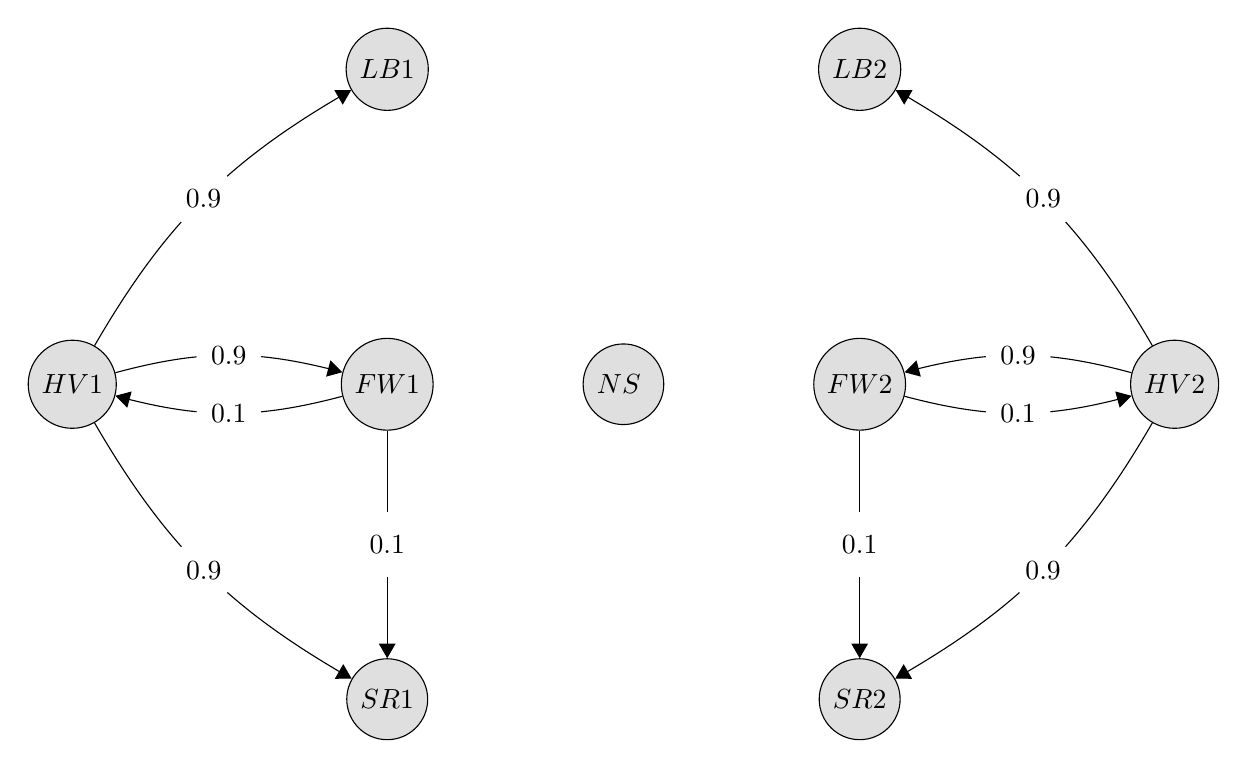
\begin{tikzpicture}[scale = 1, auto = center, every node/.style = {circle,
	draw = black, fill = gray!25}, bend angle = 90]

		\node ($NS$)  at ( 0,  8) [align = center] {{$NS$} };
		\node ($LB1$) at (-3, 12) [align = center] {{$LB1$}};
		\node ($LB2$) at ( 3, 12) [align = center] {{$LB2$}};
		\node ($FW1$) at (-3,  8) [align = center] {{$FW1$}};  
		\node ($FW2$) at ( 3,  8) [align = center] {{$FW2$}};
		\node ($HV1$) at (-7,  8) [align = center] {{$HV1$}};
		\node ($HV2$) at ( 7,  8) [align = center] {{$HV2$}};  
		\node ($SR1$) at (-3,  4) [align = center] {{$SR1$}};
		\node ($SR2$) at ( 3,  4) [align = center] {{$SR2$}};

	    \foreach \from/\phy/\to in {$HV1$/0.9/$LB1$, $HV2$/0.9/$SR2$, $HV1$/0.9/$FW1$, $FW1$/0.1/$HV1$}
	    	\path (\from) edge [-triangle 60, bend left = 15] node[fill=white, draw=none] {\phy} (\to);
	    
	    \foreach \from/\phy/\to in {$HV2$/0.9/$LB2$, $HV1$/0.9/$SR1$, $FW2$/0.1/$HV2$, $HV2$/0.9/$FW2$}
	    	\path (\from) edge [-triangle 60, bend right = 15] node[fill=white, draw=none] {\phy} (\to);
	    
	    \foreach \from/\phy/\to in {$FW1$/0.1/$SR1$, $FW2$/0.1/$SR2$}
	    	\path (\from) edge [-triangle 60] node[fill=white, draw=none] {\phy} (\to);
	
	\end{tikzpicture}
	\caption{Cloud-computing architechture}
    \label{fig:cloud}
\end{figure}

\newpage

We now consider a model depicting a cloud-computing architecture shown in
Fig~\ref{fig:cloud}. There is a solid, directed edge from component type $i$
to component type $j$ if $j \in \Gamma_i$, and the label on the edge is
$\phi_{i,j}$. The dashed, undirected edge shows the connection of our system
to the public Internet. Our system is designed to handle hypertext transfer
protocol (HTTP) requests and simple mail transfer protocol (SMTP) requests. $NS$
represents a network switch; $LB1$ and $LB2$ are two types of load
balancers; $FW1$ and $FW2$ denote two types of firewalls; $HV1$ and $HV2$ signify
two types of hypervisors; and $SR1$ and $SR2$ portray two types of server racks.
This organization of components specifically shows a firewall ``sandwich" as
described in \cite{Salch:2004}.

We set $r_{NS} = r_{LB1} = r_{LB2} = r_{FW1} = r_{FW2} = r_{HV1} = r_{HV2} =
2$ and $r_{SR1} = r_{SR2} = 3$. Let $\upsilon_i$ define the number of
components of type $i$ that need to be up for the system to remain
operational. We need at least two server racks of each type $SR1$ and $SR2$ to be
up to be able to parallel process across server racks. For other component
types, we require at least one component of each type of the system to be up
for the system to remain operational. Thus, $\upsilon_{NS} =
\upsilon_{LB1} = \upsilon_{LB2} = \upsilon_{FW1} = \upsilon_{FW2} =
\upsilon_{HV1} = \upsilon_{HV2} = 1$ and $\upsilon_{SR1} = \upsilon_{SR2} =
2$. Additionally, our system operates in two environments: high demand ($e =
0$) and low demand ($e = 1$). This gives us a state space of size 69984.
Solving this using the previous version of DECaF takes xxx
seconds, whereas using the new version's tree-generation algorithms given in
Section \ref{sec:alg} takes xxx seconds. 

We build the system such that all component types that are located to the left
of the network switch (i.e., types with a ``1" in their names) handle SMTP
requests only, whereas all component types located to the right of the network
switch (i.e., types with a ``2" in their names) handle HTTP requests only.
Thus, both the branches need to be operational for the system to be able to
handle HTTP and SMTP requests. This type of decoupling ensures that hardware
failure on one side does not immediately propagate to the other. In this model
the system-up condition is an AND of the individual-up conditions. Note that
both the previous and new versions of DECaF allow for a general boolean
combination of inequalities.

\iffalse We assume that failure of any component causes a downward-propagating
cascading failure because components on levels below the failed component end
up going offline and reach a dormant state. The propagation cannot continue
via firewalls onto server racks because although the failure of a firewall
renders server racks vulnerable, they are still ``online". To comply with our
model, dormancy is treated as a failure. We define the public Internet to be
at $depth$ 0, the network switch to be at $depth = 1$ and so on. Thus for the
downward-propagating cascading failure, $\phi_{i, \, j} = 1$ satisfying $i, j
\in \Omega, \; depth(j) = depth(i) + 1$ where $i$ and $j$ are on the same
side. \fi As stated in \cite{ReHype:2011}, ``hypervisors almost always cause
other system components to fail and certainly cause server racks to fail
because of state corruption." Thus, we assume there is probability 0.9 that a
hypervisor causes a firewall, a load balancer or a server rack to fail. A
firewall that solely implements an access-control-list verification is one
example of a vulnerable firewall. Such a firewall may let malicious packets
get through and cause a failure of a load balancer, which we assume occurs
with probability 0.5. The failure of a firewall can cause a hypervisor to fail
due to the failed firewall sending malformed packets. We assume the
probability of this is 0.1. A failed firewall in rare cases (which we model by
setting $\phi_{FW1, \, SR1} = \phi_{FW2, \, SR2} = 0.1$) can expose server
racks to attack, though most likely server racks become unusable because of a
hypervisor failure.

To estimate the component failure rates, we assume that in a high-demand
environment a component is going to fail on average in twice the time of its
warranty and in a low-demand environment a component fails in about eight
times the period of its warranty. Our time unit is hours. Typical commercial
network switches, load balancers and hypervisors have warranties of 90 days
(2160 hours). Thus, $\lambda_{NS, \, 0} = \lambda_{LB1, \, 0} =
\lambda_{LB2, \, 0} = \lambda_{HV1, \, 0} = \lambda_{HV2, \, 0} =
1 / 4320$ and $\lambda_{NS, \, 1} = \lambda_{LB1, \, 1} = \lambda_{LB2,
\, 1} = \lambda_{HV1, \, 1} = \lambda_{HV2, \, 1} = 1 / 17280$. Since
firewalls fail on average once in five years, we set $\lambda_{FW1, 0} =
\lambda_{FW2, 0} = \lambda_{FW2, 1} = \lambda_{FW1, 1} = 1 / 43800 $.
Commercial server racks often have 3-year warranties giving us $\lambda_{SR1,
\, 0} = \lambda_{SR2, \, 0} = 1 / 52560$ and $\lambda_{SR1, \, 1} =
\lambda_{SR2, \, 1} = 1 / 210240$.

For the components' repair rates, we assume that all failed hardware
components are swapped out with a repair rate of 1 regardless of the
environment, i.e., we can replace one component an hour on average. \iffalse A
repair for a hardware component may also be having to restart that part of the
system if the component is in a dormant condition. \fi Firewalls being 
non-hardware components need to be reconfigured after they fail and this occurs
with a repair rate of 0.25. Our system switches between environments once
every 12 hours on average giving us the following environment transition rates
$\nu_{0, 1} = 1 / 12$ and $\nu_{1, 0} = 1 / 12$.

\bibliographystyle{plain}
\bibliography{cloud}

\end{document}